\documentclass[11pt]{article}

\usepackage[margin=1in]{geometry}
\usepackage[T1]{fontenc}
\usepackage[utf8]{inputenc}
\usepackage{lmodern}
\usepackage{microtype}
\usepackage{amsmath, amssymb, mathtools}
\usepackage{booktabs}
\usepackage{array}
\usepackage{enumitem}
\usepackage{tikz}
\usepackage{pgfplots}
\usepackage[most]{tcolorbox}
\usepackage{hyperref}
\usepackage{fancyhdr}
\usepackage{titlesec}
\usepackage{caption}

\pgfplotsset{compat=1.18}
\usetikzlibrary{arrows.meta, positioning, shapes.geometric, calc, decorations.pathreplacing, fit}

\hypersetup{
  colorlinks=true,
  linkcolor=blue!55!black,
  urlcolor=blue!55!black,
  citecolor=blue!55!black,
  pdftitle={A Gentle Tutorial on Variational Inference},
  pdfauthor={OpenAI}
}

\pagestyle{fancy}
\fancyhf{}
\lhead{Variational Inference}
\rhead{A gentle tutorial}
\cfoot{\thepage}
\setlength{\headheight}{14pt}

\titleformat{\section}{\Large\bfseries\color{blue!50!black}}{\thesection}{0.7em}{}
\titleformat{\subsection}{\large\bfseries\color{blue!35!black}}{\thesubsection}{0.7em}{}
\titleformat{\subsubsection}{\normalsize\bfseries\color{blue!20!black}}{\thesubsubsection}{0.7em}{}

\definecolor{boxblue}{RGB}{235,244,255}
\definecolor{boxgreen}{RGB}{236,249,240}
\definecolor{boxorange}{RGB}{255,246,232}
\definecolor{boxred}{RGB}{255,238,238}
\definecolor{darkblue}{RGB}{20,70,120}

\newtcolorbox{idea}[1]{
  breakable,
  colback=boxblue,
  colframe=blue!50!black,
  title=#1,
  fonttitle=\bfseries,
  arc=2mm,
  boxrule=0.8pt
}

\newtcolorbox{examplebox}[1]{
  breakable,
  colback=boxgreen,
  colframe=green!45!black,
  title=#1,
  fonttitle=\bfseries,
  arc=2mm,
  boxrule=0.8pt
}

\newtcolorbox{warningbox}[1]{
  breakable,
  colback=boxorange,
  colframe=orange!70!black,
  title=#1,
  fonttitle=\bfseries,
  arc=2mm,
  boxrule=0.8pt
}

\newcommand{\E}{\mathbb{E}}
\newcommand{\KL}{\mathrm{KL}}
\newcommand{\data}{\mathcal{D}}
\newcommand{\given}{\,|\,}

\begin{document}
\pagenumbering{gobble}

\begin{titlepage}
\centering
\vspace*{1.1cm}
{\Huge\bfseries A Gentle Tutorial on\\[0.2cm] Variational Inference\par}
\vspace{0.35cm}
{\Large and Approximate Variational Inference\par}
\vspace{0.8cm}
{\large Written for a high school student who is new to Bayesian inference\par}
\vspace{1.1cm}

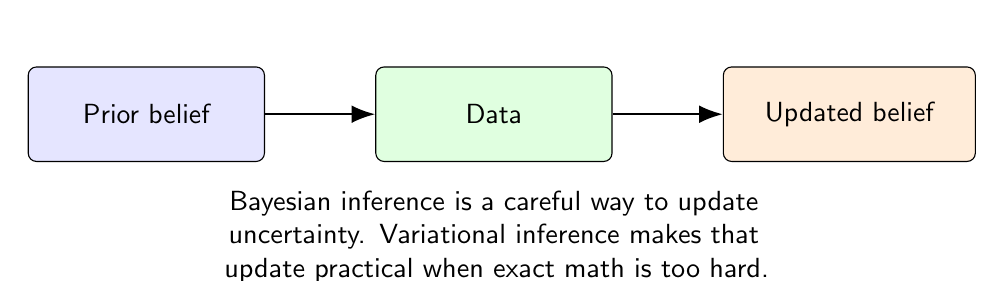
\begin{tikzpicture}[scale=1.0, every node/.style={font=\sffamily}]
  \node[draw, rounded corners=3pt, fill=blue!10, minimum width=3.0cm, minimum height=1.2cm] (prior) {Prior belief};
  \node[draw, rounded corners=3pt, fill=green!12, minimum width=3.0cm, minimum height=1.2cm, right=1.4cm of prior] (data) {Data};
  \node[draw, rounded corners=3pt, fill=orange!15, minimum width=3.2cm, minimum height=1.2cm, right=1.4cm of data] (posterior) {Updated belief};
  \draw[-{Latex[length=3mm]}, thick] (prior) -- (data);
  \draw[-{Latex[length=3mm]}, thick] (data) -- (posterior);
  \node[below=0.25cm of data, text width=7.5cm, align=center] {Bayesian inference is a careful way to update uncertainty. Variational inference makes that update practical when exact math is too hard.};
\end{tikzpicture}

\vfill
{\large \today\par}
\end{titlepage}
\pagenumbering{arabic}

\tableofcontents
\newpage

\section{The big picture}

Suppose you are trying to answer a question, but you are not completely sure.
For example:

\begin{itemize}[leftmargin=*]
  \item Is a coin fair, or is it biased toward heads?
  \item How popular is a movie before everyone has rated it?
  \item What is the most likely path of a robot if its sensors are noisy?
  \item Which topic is an article about if some words are missing?
\end{itemize}

Bayesian inference gives us a way to use probability to represent uncertainty.
Instead of giving one answer, Bayesian inference gives a whole distribution of possible answers.
A distribution is like a map that says which answers are more likely and which are less likely.

\begin{idea}{Main idea}
Bayesian inference asks: 
\[
\text{What should I believe after seeing the data?}
\]
Variational inference asks:
\[
\text{Can I find an easier distribution that is close enough to the true Bayesian answer?}
\]
\end{idea}

People often shorten \textbf{variational inference} to \textbf{VI}. The phrase \textbf{approximate variational inference} usually means the same general approach, with the reminder that the answer is an approximation.
The word ``variational'' means that we choose a family of possible distributions and vary its parameters until it fits well.

\section{A tiny amount of probability background}

A \textbf{random variable} is a quantity whose value is uncertain. If $\theta$ is the probability that a coin lands heads, then $\theta$ is a number between $0$ and $1$.

A \textbf{probability distribution} describes uncertainty. For a coin bias $\theta$, a distribution might say:

\begin{itemize}[leftmargin=*]
  \item values near $0.5$ are likely if we think the coin is fair;
  \item values near $0.9$ are likely if we think the coin usually lands heads;
  \item many values are possible if we are not sure yet.
\end{itemize}

\subsection{Bayes' rule}

Bayes' rule is the central formula:

\begin{equation}
\boxed{
  p(\theta \given \data)
  = \frac{p(\data \given \theta)p(\theta)}{p(\data)}
}
\end{equation}

Here is what each part means.

\begin{center}
\renewcommand{\arraystretch}{1.25}
\begin{tabular}{>{\raggedright\arraybackslash}p{0.23\textwidth} >{\raggedright\arraybackslash}p{0.64\textwidth}}
\toprule
Symbol & Meaning \\
\midrule
$p(\theta)$ & The \textbf{prior}: what we believe before seeing the data. \\
$p(\data \given \theta)$ & The \textbf{likelihood}: how well a value of $\theta$ explains the observed data. \\
$p(\theta \given \data)$ & The \textbf{posterior}: what we believe after seeing the data. \\
$p(\data)$ & The \textbf{evidence}: a normalizing number that makes the posterior add up to $1$. \\
\bottomrule
\end{tabular}
\end{center}

\begin{idea}{Bayes' rule in words}
\[
\text{posterior} = \frac{\text{likelihood} \times \text{prior}}{\text{evidence}}.
\]
The prior says what seemed reasonable before the data. The likelihood rewards explanations that make the data look likely. The evidence makes the final result a valid probability distribution.
\end{idea}

\section{A simple coin example}

Imagine we flip a coin $10$ times and get $7$ heads and $3$ tails.
Let $\theta$ be the unknown chance of heads.

Before seeing the flips, suppose we use a prior that says the coin is probably not extremely biased, but we are still uncertain. One convenient choice is called a Beta distribution:

\[
\theta \sim \mathrm{Beta}(2,2).
\]

You do not need to memorize the Beta distribution. For now, just remember that it is a distribution over numbers between $0$ and $1$, so it is useful for probabilities like a coin bias.

After observing $7$ heads and $3$ tails, Bayes' rule gives:

\[
\theta \given \data \sim \mathrm{Beta}(2+7, 2+3) = \mathrm{Beta}(9,5).
\]

The posterior mean is:

\[
\E[\theta \given \data] = \frac{9}{9+5} = \frac{9}{14} \approx 0.64.
\]

So after seeing the data, our best average guess is that the coin lands heads about $64\%$ of the time. But the posterior distribution also tells us how uncertain we still are.

\begin{figure}[h]
\centering
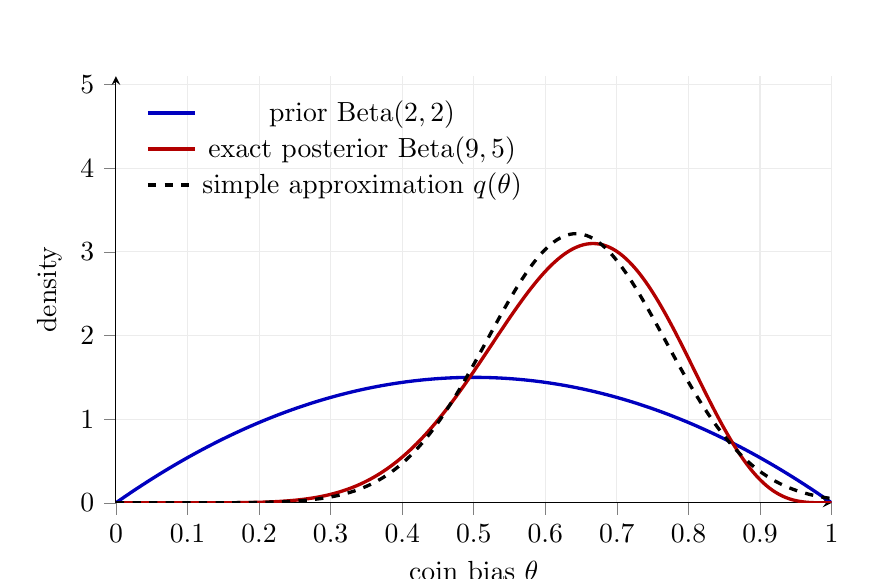
\begin{tikzpicture}
\begin{axis}[
  width=0.88\textwidth,
  height=7cm,
  axis lines=left,
  xmin=0, xmax=1,
  ymin=0, ymax=5.1,
  xlabel={coin bias $\theta$},
  ylabel={density},
  legend style={draw=none, fill=none, at={(0.03,0.97)}, anchor=north west},
  tick align=outside,
  samples=220,
  domain=0:1,
  grid=both,
  grid style={gray!15}
]
\addplot[blue!75!black, very thick] {6*x*(1-x)};
\addlegendentry{prior $\mathrm{Beta}(2,2)$}
\addplot[red!70!black, very thick] {6435*x^8*(1-x)^4};
\addlegendentry{exact posterior $\mathrm{Beta}(9,5)$}
\addplot[black, very thick, dashed] {1/(0.124*sqrt(2*pi))*exp(-((x-0.643)^2)/(2*0.124^2))};
\addlegendentry{simple approximation $q(\theta)$}
\end{axis}
\end{tikzpicture}
\caption{Bayesian updating for a coin. The posterior is more concentrated than the prior because we learned from data. The dashed curve is a simple approximation to the posterior.}
\end{figure}

\begin{examplebox}{What this picture teaches}
The blue curve is our belief before data. The red curve is our belief after data. The dashed curve is not exactly correct, but it is easier to work with. Variational inference is about finding a dashed curve that is as close as possible to the true red curve.
\end{examplebox}

\section{Why exact Bayesian inference can be hard}

In the coin example, the math worked nicely. But many real problems have many unknowns.
For example, a model might have thousands or millions of hidden variables.

Bayes' rule still says:

\[
p(z \given x) = \frac{p(x,z)}{p(x)},
\]

where:

\begin{itemize}[leftmargin=*]
  \item $x$ means the observed data;
  \item $z$ means hidden variables we want to infer;
  \item $p(x,z)$ is the joint probability of data and hidden variables;
  \item $p(z \given x)$ is the posterior distribution.
\end{itemize}

The hard part is often the denominator:

\begin{equation}
\boxed{
  p(x) = \int p(x,z)\,dz
}
\end{equation}

If you have not seen integrals before, think of the integral as adding up all possible hidden explanations $z$.
If there are many hidden variables, this can be like trying to add up the heights of a mountain range in thousands of dimensions.
That is usually impossible to do exactly.

\begin{warningbox}{The bottleneck}
The posterior $p(z \given x)$ is often hard because the evidence $p(x)$ requires adding over every possible hidden explanation. Variational inference avoids computing this hard quantity directly.
\end{warningbox}

\section{The variational inference idea}

Instead of trying to compute the exact posterior $p(z \given x)$, VI chooses a simpler distribution $q(z)$ and tries to make it close to the true posterior.

\begin{equation}
\boxed{
  p(z \given x) \quad \text{is hard, so use} \quad q(z) \approx p(z \given x).
}
\end{equation}

The distribution $q$ is called the \textbf{variational distribution}.
It usually has parameters, which we can call $\lambda$:

\[
q(z) = q(z;\lambda).
\]

For example:

\begin{itemize}[leftmargin=*]
  \item If $q$ is a normal distribution, $\lambda$ might include a mean $\mu$ and standard deviation $\sigma$.
  \item If $q$ is a Beta distribution, $\lambda$ might include two shape numbers $a$ and $b$.
  \item If $q$ is a product of many simple distributions, $\lambda$ might include many means and variances.
\end{itemize}

\begin{figure}[h]
\centering
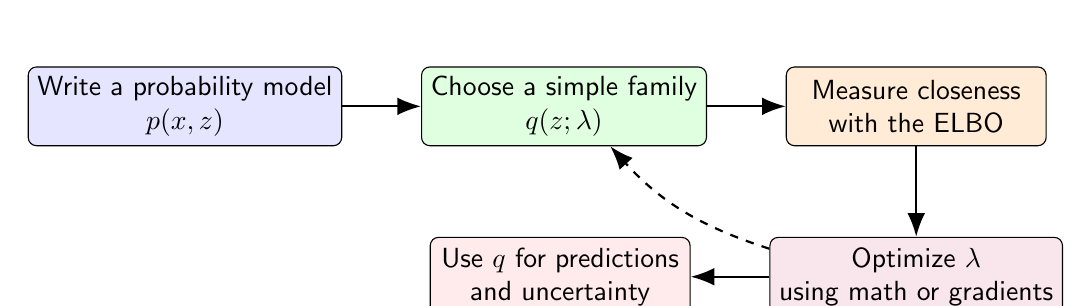
\begin{tikzpicture}[node distance=1.15cm and 1.0cm, every node/.style={font=\sffamily}]
  \tikzstyle{stepbox}=[draw, rounded corners=3pt, align=center, minimum width=3.3cm, minimum height=1.0cm]
  \node[stepbox, fill=blue!10] (model) {Write a probability model\\$p(x,z)$};
  \node[stepbox, fill=green!12, right=of model] (family) {Choose a simple family\\$q(z;\lambda)$};
  \node[stepbox, fill=orange!16, right=of family] (objective) {Measure closeness\\with the ELBO};
  \node[stepbox, fill=purple!10, below=of objective] (opt) {Optimize $\lambda$\\using math or gradients};
  \node[stepbox, fill=red!8, left=of opt] (use) {Use $q$ for predictions\\and uncertainty};
  \draw[-{Latex[length=3mm]}, thick] (model) -- (family);
  \draw[-{Latex[length=3mm]}, thick] (family) -- (objective);
  \draw[-{Latex[length=3mm]}, thick] (objective) -- (opt);
  \draw[-{Latex[length=3mm]}, thick] (opt) -- (use);
  \draw[-{Latex[length=3mm]}, thick, dashed] (opt) to[bend left=15] (family);
\end{tikzpicture}
\caption{The basic variational inference workflow. The dashed arrow reminds us that optimization repeatedly adjusts the parameters of $q$.}
\end{figure}

\section{How do we measure ``close''? KL divergence}

To choose the best $q$, we need a way to measure how different two distributions are.
A common choice is called \textbf{KL divergence}, short for Kullback-Leibler divergence.

For VI, the important form is:

\begin{equation}
\KL(q(z)\,\|\,p(z \given x))
= \E_{q}\left[\log \frac{q(z)}{p(z \given x)}\right].
\end{equation}

This means:

\begin{itemize}[leftmargin=*]
  \item draw possible hidden values $z$ from the easy distribution $q$;
  \item compare how much probability $q$ gives to those values versus the true posterior;
  \item average that comparison.
\end{itemize}

\begin{idea}{Intuition for KL divergence}
KL divergence is $0$ when the two distributions match perfectly. It is positive when they differ. Smaller is better.
\end{idea}

So the dream would be:

\[
q^*(z) = \arg\min_{q} \KL(q(z)\,\|\,p(z \given x)).
\]

The notation $\arg\min$ means ``the choice that makes this as small as possible.''

\subsection{A small warning about KL}

KL divergence is not exactly the same as ordinary distance. In particular:

\[
\KL(q\|p) \ne \KL(p\|q).
\]

Changing the order changes the behavior. Many VI methods use $\KL(q\|p)$, which can sometimes focus on one high-probability region and ignore other possible regions. This is one reason VI can be fast but sometimes overconfident.

\section{The ELBO: the objective VI actually maximizes}

There is a problem: the KL formula contains the true posterior $p(z \given x)$, which is exactly what we do not know.
So how can we minimize it?

The trick is to use a related quantity called the \textbf{evidence lower bound}, usually shortened to \textbf{ELBO}.

\begin{equation}
\boxed{
\mathcal{L}(q)
= \E_q[\log p(x,z)] - \E_q[\log q(z)].
}
\end{equation}

The symbol $\mathcal{L}$ is just a name for the ELBO.

A very important identity is:

\begin{equation}
\boxed{
\log p(x) = \mathcal{L}(q) + \KL(q(z)\,\|\,p(z \given x)).
}
\end{equation}

Since KL divergence is always at least $0$, we get:

\[
\mathcal{L}(q) \le \log p(x).
\]

That is why it is called a lower bound: the ELBO is below the true log evidence.

\begin{figure}[h]
\centering
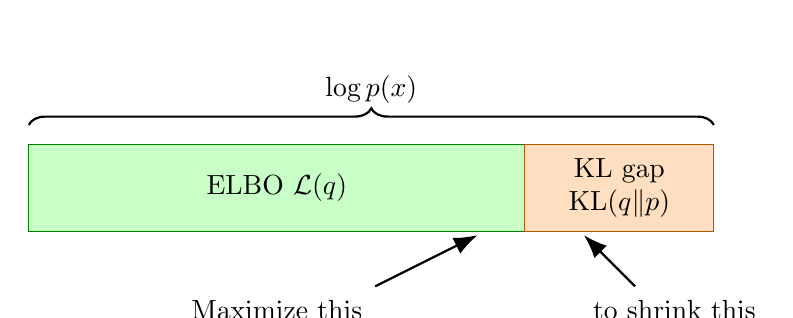
\begin{tikzpicture}[x=1cm,y=1cm]
  \draw[fill=green!22, draw=green!50!black] (0,0) rectangle (6.3,1.1);
  \draw[fill=orange!25, draw=orange!70!black] (6.3,0) rectangle (8.7,1.1);
  \node at (3.15,0.55) {ELBO $\mathcal{L}(q)$};
  \node[align=center] at (7.5,0.55) {KL gap\\$\KL(q\|p)$};
  \draw[decorate, decoration={brace, amplitude=6pt}, thick] (0,1.35) -- (8.7,1.35) node[midway, yshift=0.45cm] {$\log p(x)$};
  \draw[-{Latex[length=3mm]}, thick] (4.4,-0.7) -- (5.7,-0.05);
  \node[align=center] at (3.15,-1.0) {Maximize this};
  \draw[-{Latex[length=3mm]}, thick] (7.7,-0.7) -- (7.05,-0.05);
  \node[align=center] at (8.2,-1.0) {to shrink this};
\end{tikzpicture}
\caption{The log evidence is split into the ELBO plus a KL gap. Since $\log p(x)$ is fixed for the data, increasing the ELBO decreases the KL gap.}
\end{figure}

\begin{idea}{The key trick}
We cannot directly minimize $\KL(q\|p)$ because the true posterior is hard.
But we can maximize the ELBO, and that automatically makes $q$ closer to the posterior.
\end{idea}

\subsection{Another useful form of the ELBO}

If the model has a prior $p(z)$ and a likelihood $p(x\given z)$, then:

\[
p(x,z) = p(x\given z)p(z).
\]

The ELBO can be written as:

\begin{equation}
\boxed{
\mathcal{L}(q)
= \E_q[\log p(x\given z)] - \KL(q(z)\,\|\,p(z)).
}
\end{equation}

This version is easy to understand:

\begin{itemize}[leftmargin=*]
  \item $\E_q[\log p(x\given z)]$ rewards hidden explanations $z$ that explain the data well.
  \item $\KL(q(z)\|p(z))$ penalizes $q$ if it moves too far away from the prior.
\end{itemize}

So VI balances two goals: explain the data, but do not become needlessly complicated.

\section{Mean-field variational inference}

One of the most common simplifications is called the \textbf{mean-field assumption}.
Suppose the hidden variables are:

\[
z = (z_1,z_2,\ldots,z_m).
\]

Mean-field VI assumes the approximation factors into separate pieces:

\begin{equation}
\boxed{
q(z_1,z_2,\ldots,z_m) = q_1(z_1)q_2(z_2)\cdots q_m(z_m).
}
\end{equation}

In words, mean-field VI pretends the hidden variables are independent under $q$.
This is often not exactly true, but it makes the math and computation much easier.

\begin{figure}[h]
\centering
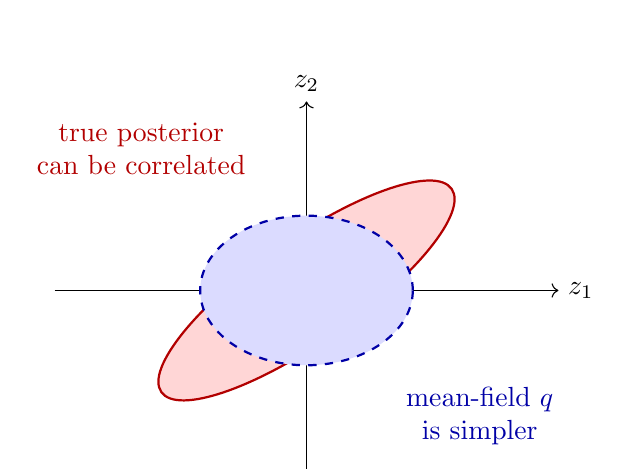
\begin{tikzpicture}[scale=1.0]
  \draw[->] (-3.2,0) -- (3.2,0) node[right] {$z_1$};
  \draw[->] (0,-2.4) -- (0,2.4) node[above] {$z_2$};
  \begin{scope}[rotate=35]
    \draw[fill=red!16, draw=red!70!black, thick] (0,0) ellipse (2.25 and 0.65);
  \end{scope}
  \draw[fill=blue!14, draw=blue!65!black, thick, dashed] (0,0) ellipse (1.35 and 0.95);
  \node[red!70!black, align=center] at (-2.1,1.8) {true posterior\\can be correlated};
  \node[blue!65!black, align=center] at (2.2,-1.6) {mean-field $q$\\is simpler};
\end{tikzpicture}
\caption{A cartoon of mean-field VI. The true posterior might have correlation, shown by the tilted red ellipse. The mean-field approximation is simpler and axis-aligned, shown by the dashed blue ellipse.}
\end{figure}

\subsection{Coordinate ascent idea}

In some models, we can update one part of $q$ at a time.
The best update for one factor has the form:

\begin{equation}
\boxed{
\log q_i^*(z_i)
= \E_{q_{-i}}[\log p(x,z)] + \text{constant}.
}
\end{equation}

This formula looks advanced, but the idea is simple:

\begin{itemize}[leftmargin=*]
  \item update $q_i$ while holding the other pieces fixed;
  \item use the average effect of the other variables;
  \item repeat until the ELBO stops improving much.
\end{itemize}

This method is called \textbf{coordinate ascent variational inference}, or \textbf{CAVI}.

\section{Worked example: a one-number Gaussian model}

The coin example used a probability between $0$ and $1$.
Now let us use an example where the unknown number can be any real number.

Suppose $\theta$ is an unknown quantity, such as a student's true skill level on a test scale.
Before seeing a measurement, we use the prior:

\[
\theta \sim \mathcal{N}(0,1).
\]

This says $\theta$ is probably near $0$, but it could be positive or negative.
Now suppose we observe one noisy measurement:

\[
x = 2.
\]

The measurement model is:

\[
x \given \theta \sim \mathcal{N}(\theta,1).
\]

This says the observation is centered around the true $\theta$, but there is noise.

\subsection{Choose a variational family}

Choose a normal approximation:

\[
q(\theta) = \mathcal{N}(m,s^2).
\]

The variational parameters are $m$ and $s^2$:

\begin{itemize}[leftmargin=*]
  \item $m$ controls the center of the approximation;
  \item $s^2$ controls the uncertainty.
\end{itemize}

For this model, the ELBO can be simplified to:

\begin{equation}
\mathcal{L}(m,s^2)
= -\frac{1}{2}\left[(2-m)^2+s^2\right]
  -\frac{1}{2}\left[s^2+m^2-1-\log(s^2)\right]
  + \text{constant}.
\end{equation}

Do not worry about every algebra step. The important point is that this is now just an optimization problem over two numbers, $m$ and $s^2$.

Maximizing this expression gives:

\[
\boxed{m=1, \qquad s^2=\frac{1}{2}.}
\]

So the best variational approximation is:

\[
q(\theta)=\mathcal{N}\left(1,\frac{1}{2}\right).
\]

In this special example, the exact posterior is also:

\[
p(\theta\given x)=\mathcal{N}\left(1,\frac{1}{2}\right).
\]

So VI finds the exact answer because our chosen family was flexible enough to contain the true posterior.

\begin{examplebox}{Lesson from this example}
VI turns Bayesian inference into optimization. Instead of directly solving for the full posterior, we choose a simpler shape $q$ and tune its parameters to maximize the ELBO.
\end{examplebox}

\section{How approximate variational inference works in practice}

In small textbook examples, we may be able to write the ELBO exactly and solve it by hand.
In modern machine learning, the model may be too complicated for that.
Then we use approximate numerical methods.

A typical practical VI algorithm looks like this:

\begin{enumerate}[leftmargin=*]
  \item Choose a variational family $q(z;\lambda)$.
  \item Write the ELBO $\mathcal{L}(\lambda)$.
  \item Estimate the ELBO or its gradient using samples.
  \item Use an optimizer, such as gradient descent, to improve $\lambda$.
  \item Stop when the ELBO is no longer improving much.
\end{enumerate}

\subsection{Sampling estimates}

Sometimes the expectation

\[
\E_q[\log p(x,z)]
\]

is hard to compute exactly. We can estimate it by drawing samples from $q$.
For example, if we draw $S$ samples $z^{(1)},\ldots,z^{(S)}$ from $q$, then:

\[
\E_q[\log p(x,z)] \approx \frac{1}{S}\sum_{s=1}^S \log p(x,z^{(s)}).
\]

This is just an average. More samples usually give a more accurate estimate, but they take more time.

\subsection{Gradient descent idea}

A gradient tells us which direction increases a function the fastest.
If $\lambda$ represents the parameters of $q$, gradient ascent updates them like this:

\[
\lambda_{\text{new}}
= \lambda_{\text{old}} + \eta \nabla_{\lambda}\mathcal{L}(\lambda).
\]

Here $\eta$ is the learning rate, a small positive number that controls the step size.
This is called gradient \emph{ascent} because we want to make the ELBO bigger.

\subsection{The reparameterization trick}

For normal distributions, a useful trick is:

\[
z \sim \mathcal{N}(\mu,\sigma^2)
\quad \Longleftrightarrow \quad
z = \mu + \sigma\epsilon, \qquad \epsilon \sim \mathcal{N}(0,1).
\]

This separates the randomness $\epsilon$ from the parameters $\mu$ and $\sigma$.
That makes it easier for computers to calculate gradients.
This trick is very important in many modern VI methods, including variational autoencoders.

\section{A simple pseudo-code recipe}

\begin{examplebox}{Variational inference pseudo-code}
\begin{enumerate}[leftmargin=*]
  \item Start with random or reasonable variational parameters $\lambda$.
  \item Repeat:
  \begin{enumerate}
    \item Draw samples $z$ from $q(z;\lambda)$, or compute expectations exactly if possible.
    \item Estimate the ELBO $\mathcal{L}(\lambda)$ and its gradient.
    \item Move $\lambda$ in the direction that increases the ELBO.
  \end{enumerate}
  \item Return $q(z;\lambda)$ as the approximate posterior.
\end{enumerate}
\end{examplebox}

\begin{figure}[h]
\centering
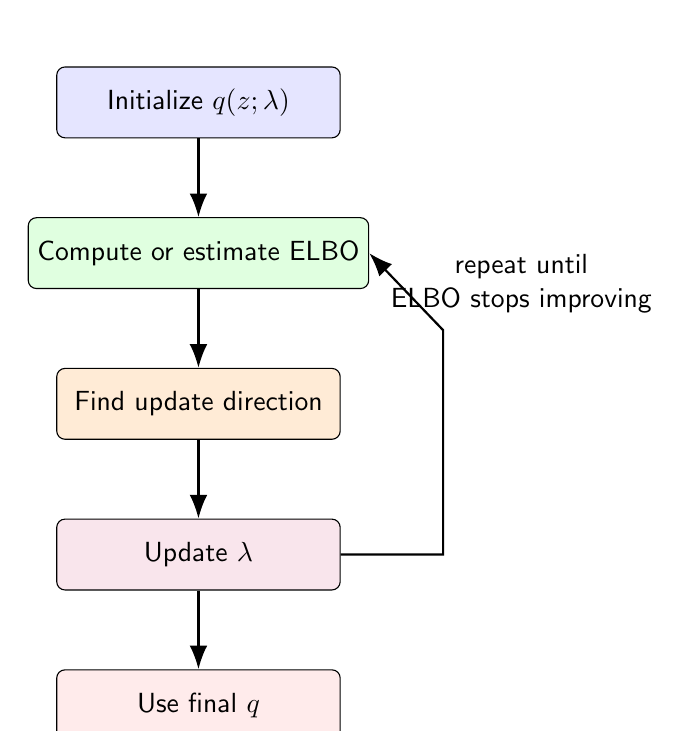
\begin{tikzpicture}[node distance=1.0cm, every node/.style={font=\sffamily}]
  \tikzstyle{box}=[draw, rounded corners=3pt, align=center, minimum width=3.6cm, minimum height=0.9cm]
  \node[box, fill=blue!10] (init) {Initialize $q(z;\lambda)$};
  \node[box, fill=green!12, below=of init] (elbo) {Compute or estimate ELBO};
  \node[box, fill=orange!16, below=of elbo] (grad) {Find update direction};
  \node[box, fill=purple!10, below=of grad] (update) {Update $\lambda$};
  \node[box, fill=red!8, below=of update] (done) {Use final $q$};
  \draw[-{Latex[length=3mm]}, thick] (init) -- (elbo);
  \draw[-{Latex[length=3mm]}, thick] (elbo) -- (grad);
  \draw[-{Latex[length=3mm]}, thick] (grad) -- (update);
  \draw[-{Latex[length=3mm]}, thick] (update.east) -- ++(1.3,0) -- ++(0,2.85) -- (elbo.east);
  \draw[-{Latex[length=3mm]}, thick] (update) -- (done);
  \node[align=center] at (4.1,-2.3) {repeat until\\ELBO stops improving};
\end{tikzpicture}
\caption{A practical VI loop. The algorithm repeatedly improves the approximate posterior.}
\end{figure}

\section{What does ``approximate'' mean?}

The word approximate appears for several reasons.

\begin{enumerate}[leftmargin=*]
  \item \textbf{The variational family may be too simple.} A normal distribution cannot perfectly match every possible posterior shape.
  \item \textbf{Mean-field assumptions may ignore relationships.} If two hidden variables are strongly linked, forcing independence can lose information.
  \item \textbf{Optimization may stop early or get stuck.} The ELBO may have many hills, and an optimizer might find a good hill but not the best hill.
  \item \textbf{Sampling adds noise.} If we estimate the ELBO using samples, the estimate is not exact.
\end{enumerate}

\begin{warningbox}{Important limitation}
VI is usually faster than many exact or sampling-based Bayesian methods, but it can underestimate uncertainty. In other words, it may be too confident.
\end{warningbox}

\section{VI compared with other Bayesian methods}

Another popular Bayesian approach is \textbf{Markov chain Monte Carlo}, usually called \textbf{MCMC}.
MCMC tries to draw samples from the true posterior. VI tries to find a simpler distribution close to the posterior.

\begin{center}
\renewcommand{\arraystretch}{1.25}
\begin{tabular}{>{\raggedright\arraybackslash}p{0.27\textwidth} >{\raggedright\arraybackslash}p{0.31\textwidth} >{\raggedright\arraybackslash}p{0.31\textwidth}}
\toprule
Method & Main idea & Usual tradeoff \\
\midrule
Exact Bayesian inference & Compute the posterior exactly. & Beautiful when possible, but often impossible for large models. \\
MCMC & Use random sampling to approximate the true posterior. & Often accurate, but can be slow. \\
Variational inference & Use optimization to find a simpler approximate posterior. & Often fast, but may be less accurate or too confident. \\
\bottomrule
\end{tabular}
\end{center}

\section{A second look at the coin example through VI}

In the coin example, the exact posterior was $\mathrm{Beta}(9,5)$.
But suppose we did not want to use a Beta posterior directly.
We could choose a simple family $q(\theta)$, such as a normal-shaped curve centered at $\mu$ with spread $\sigma$.
Then VI would try to choose $\mu$ and $\sigma$ so that:

\[
q(\theta;\mu,\sigma) \approx p(\theta\given \data).
\]

The dashed curve in Figure 1 is one such approximation.
It is not perfect because a normal distribution technically allows values less than $0$ and greater than $1$, while a coin bias must stay between $0$ and $1$.
A more careful version could use a transformed normal distribution or choose a Beta variational family.

\begin{idea}{Choosing the family matters}
If $q$ is too simple, VI can only give a rough approximation. If $q$ is flexible, VI can be more accurate but may be harder to optimize.
\end{idea}

\section{Common words you will see}

\begin{center}
\renewcommand{\arraystretch}{1.25}
\begin{tabular}{>{\raggedright\arraybackslash}p{0.26\textwidth} >{\raggedright\arraybackslash}p{0.63\textwidth}}
\toprule
Word & Meaning \\
\midrule
Prior & Belief before seeing data. \\
Likelihood & How likely the observed data is under a possible explanation. \\
Posterior & Belief after seeing data. \\
Evidence & The probability of the data under the whole model; often hard to compute. \\
Latent variable & A hidden variable we do not observe directly. \\
Variational family & The set of possible approximating distributions $q$. \\
ELBO & The objective VI maximizes. Bigger ELBO means a better approximation. \\
KL divergence & A measure of mismatch between two distributions. \\
Mean-field & An assumption that the approximate posterior factors into independent pieces. \\
Gradient ascent & A method for increasing a function step by step. \\
\bottomrule
\end{tabular}
\end{center}

\section{Mini exercises}

Try these to check your understanding.

\begin{enumerate}[leftmargin=*]
  \item In your own words, what is the difference between a prior and a posterior?
  \item Why is the evidence $p(x)$ often hard to compute?
  \item What does the variational distribution $q(z)$ try to approximate?
  \item If maximizing the ELBO makes the KL gap smaller, why do we maximize the ELBO instead of minimizing the KL directly?
  \item Suppose a coin has prior $\mathrm{Beta}(1,1)$ and you observe $8$ heads and $2$ tails. What is the posterior Beta distribution? What is its mean?
\end{enumerate}

\subsection*{Answers}

\begin{enumerate}[leftmargin=*]
  \item The prior is before data; the posterior is after data.
  \item It requires adding or integrating over many possible hidden explanations.
  \item It tries to approximate the true posterior $p(z\given x)$.
  \item The KL contains the unknown true posterior and hard evidence. The ELBO can often be computed or estimated without directly computing the evidence.
  \item The posterior is $\mathrm{Beta}(1+8,1+2)=\mathrm{Beta}(9,3)$. Its mean is $9/(9+3)=0.75$.
\end{enumerate}

\section{One-page summary}

\begin{idea}{Bayesian inference}
Use Bayes' rule to update uncertainty:
\[
p(z\given x)=\frac{p(x,z)}{p(x)}.
\]
The posterior $p(z\given x)$ is the main object we want.
\end{idea}

\begin{idea}{Why VI is needed}
The evidence
\[
p(x)=\int p(x,z)\,dz
\]
can be too hard to compute exactly, especially with many hidden variables.
\end{idea}

\begin{idea}{Variational inference}
Pick a simpler distribution $q(z;\lambda)$ and tune $\lambda$ so that:
\[
q(z;\lambda) \approx p(z\given x).
\]
\end{idea}

\begin{idea}{ELBO}
Maximize:
\[
\mathcal{L}(q)=\E_q[\log p(x,z)]-\E_q[\log q(z)].
\]
Because:
\[
\log p(x)=\mathcal{L}(q)+\KL(q\|p).
\]
Since $\log p(x)$ is fixed, making the ELBO bigger makes the KL gap smaller.
\end{idea}

\begin{idea}{Approximate VI in practice}
For complex models, computers estimate expectations with samples and improve $q$ using gradient methods. The result is usually fast and useful, but approximate.
\end{idea}

\section*{Closing thought}

A good way to remember VI is:

\begin{center}
\Large
\textbf{Bayesian inference gives the target. VI gives a practical shortcut.}
\end{center}

The target is the true posterior. The shortcut is a simpler distribution $q$ found by optimization. The art of VI is choosing a good family $q$, a good objective, and a reliable optimization method.

\end{document}
